\documentclass[svgnames,smaller,table]{beamer}
\usepackage{multirow}

\usetheme{ufmg}
\setbeamercolor*{normal text}{fg=black}
% -----------------------------------------------------------------------------------------------------------------

\title[Defesa de tese]{Acoplamento neutrônico e termo-hidráulico usando os
  códigos milonga e OpenFOAM: uma abordagem com \textit{software} livre}
\author{Vitor Vasconcelos Araújo Silva}
\date{19 de dezembro de 2016}
%\data{\today}
%\orientador{Cláubia Pereira Bezerra Lima}
%\coorientador{André Augusto Campagnole dos Santos}
\institute{%
  Universidade Federal de Minas Gerais -- UFMG
  \par
  Departamento de Engenharia Nuclear
  \par
  Programa de Pós-Graduação em Ciências e Técnicas Nucleares}

\begin{document}

%-------------------------------------------------
\begin{frame}
\titlepage
\end{frame}

%-------------------------------------------------
\begin{frame}
  \frametitle{Sumário}
  \tableofcontents%[pausesections]
\end{frame}

%-------------------------------------------------
\section{Resultados}
\begin{frame}
  \frametitle{Resultados}
  \begin{itemize}
  \item Sistema acoplado funcional
  \item Malha idêntica
  \item Baseado em \textit{software} livre
  \end{itemize}
\end{frame}

%-------------------------------------------------
\subsection{Gráficos}
\begin{frame}
  \frametitle{Resultados}
  \framesubtitle{Fluxo neutrônico: distribuição axial ($7,93 kW$)}
  %  Fluxo [$\phi/phi_{avg}$].
  \centering\includegraphics[width=\textwidth, height=7.0cm]{../figuras/Flux_rel_z_200_port.png}
  \label{fig:flux200z}
\end{frame}

%-------------------------------------------------
\subsection{Gráficos}
\begin{frame}
  \frametitle{Resultados}
  \framesubtitle{Fluxo neutrônico: distribuição radial ($7,93 kW$)}
%  Fluxo [$\phi/phi_{avg}$].
  \centering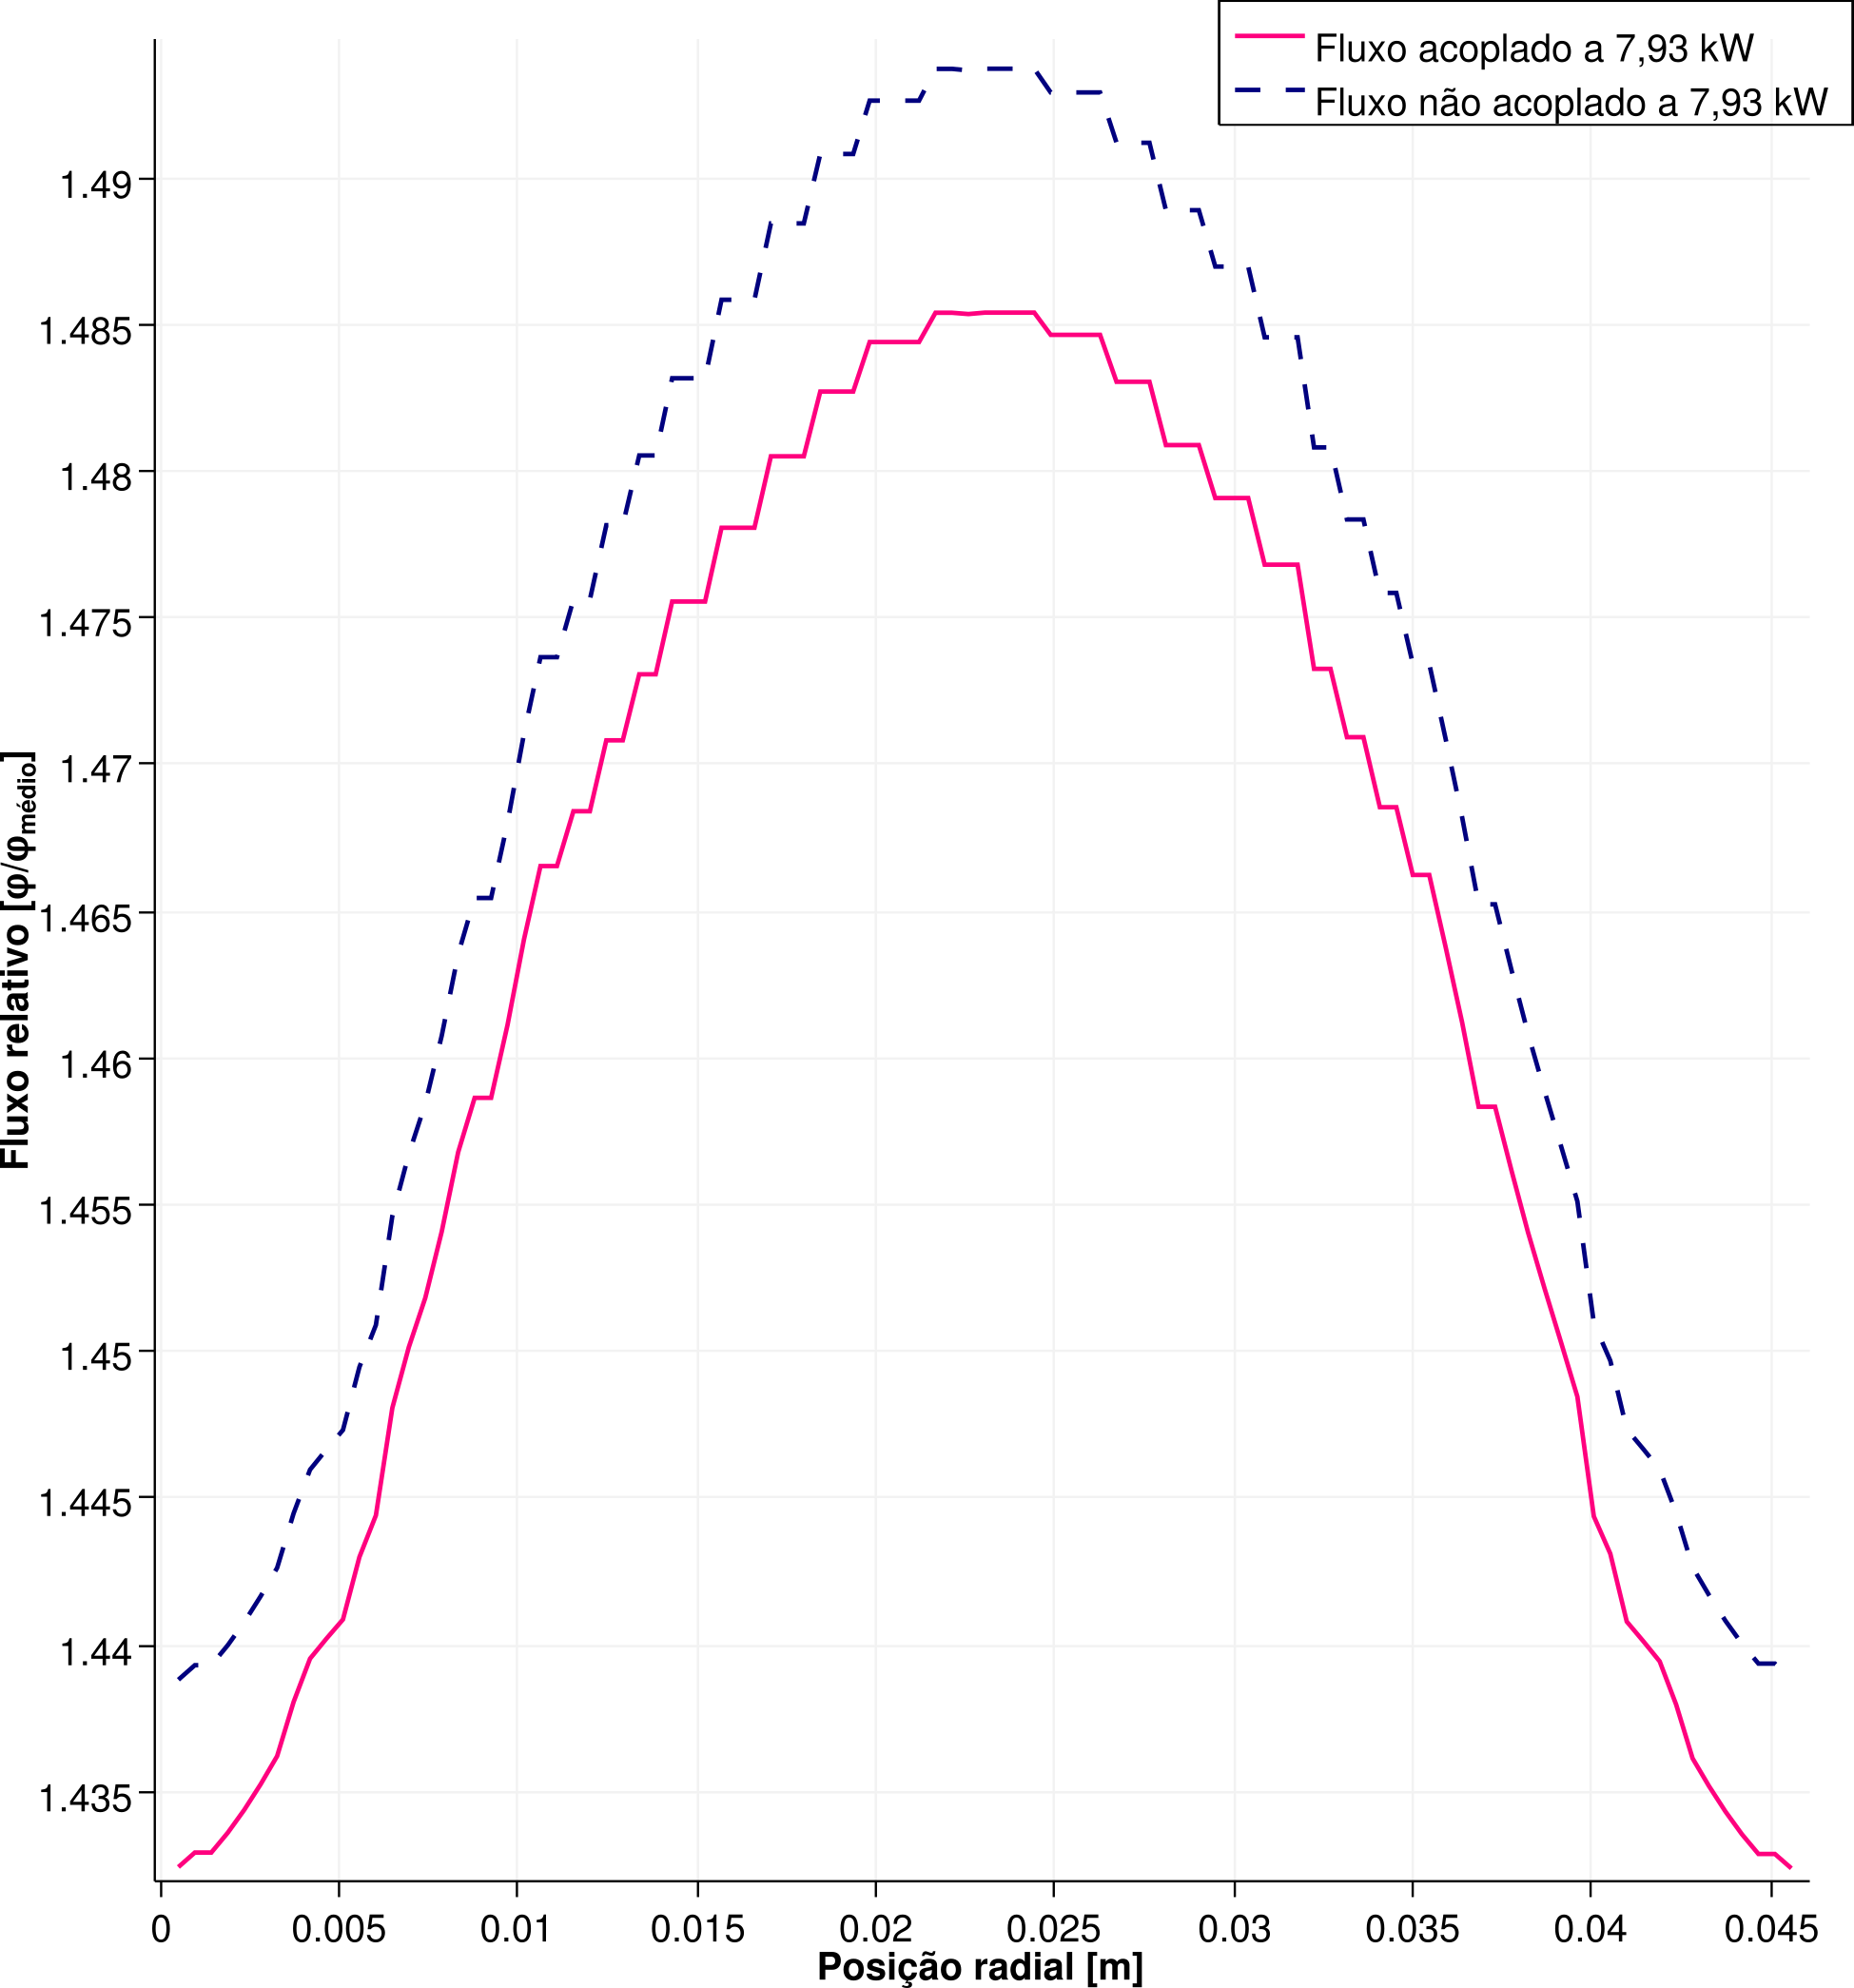
\includegraphics[width=\textwidth, height=7.0cm]{../figuras/Flux_rel_x_200_port.png}
  \label{fig:flux200x}
\end{frame}

%-------------------------------------------------
\subsection{Gráficos}
\begin{frame}
  \frametitle{Resultados}
  \framesubtitle{Potência: distribuição axial}
%  Distribuição de potência [$kW/m^3$].
  \centering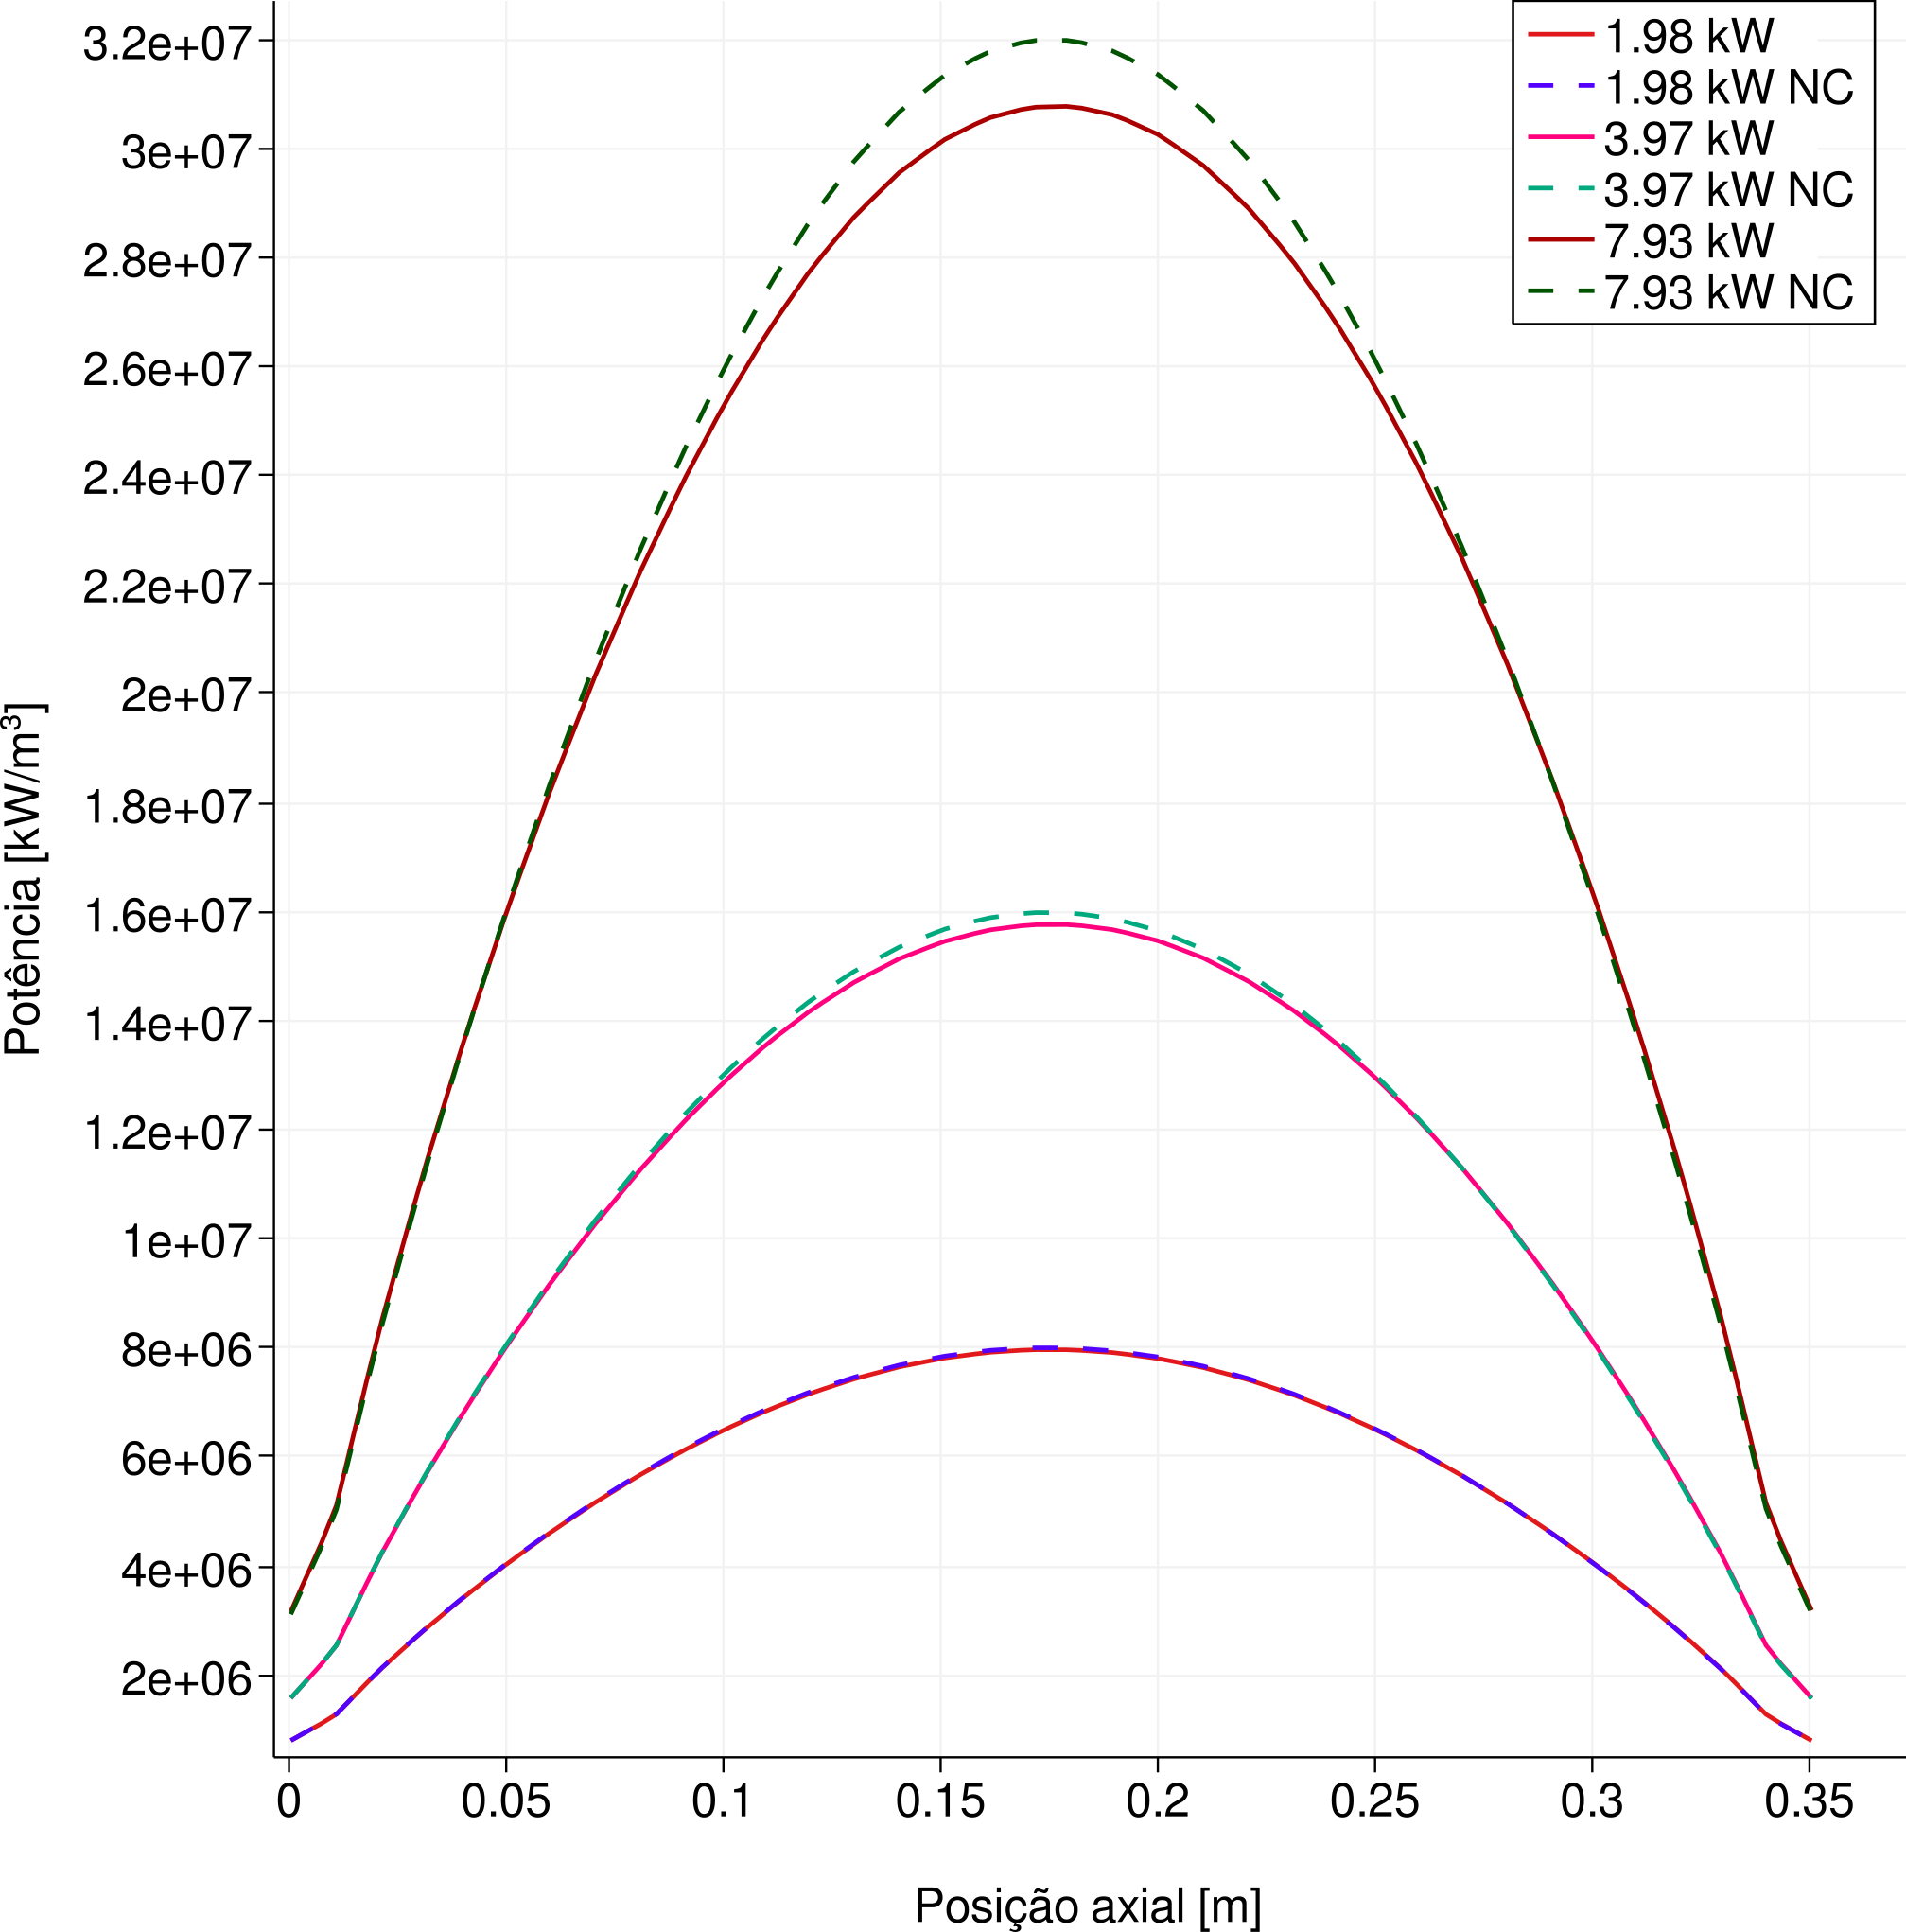
\includegraphics[width=\textwidth, height=7.0cm]{../figuras/Q_all_z_square_port.png}
  \label{fig:keff50}
\end{frame}

%-------------------------------------------------
\subsection{Gráficos}
\begin{frame}
  \frametitle{Resultados}
  \framesubtitle{Potência: distribuição radial}
%  Distribuição de potência [$KW/m^3$].
  \centering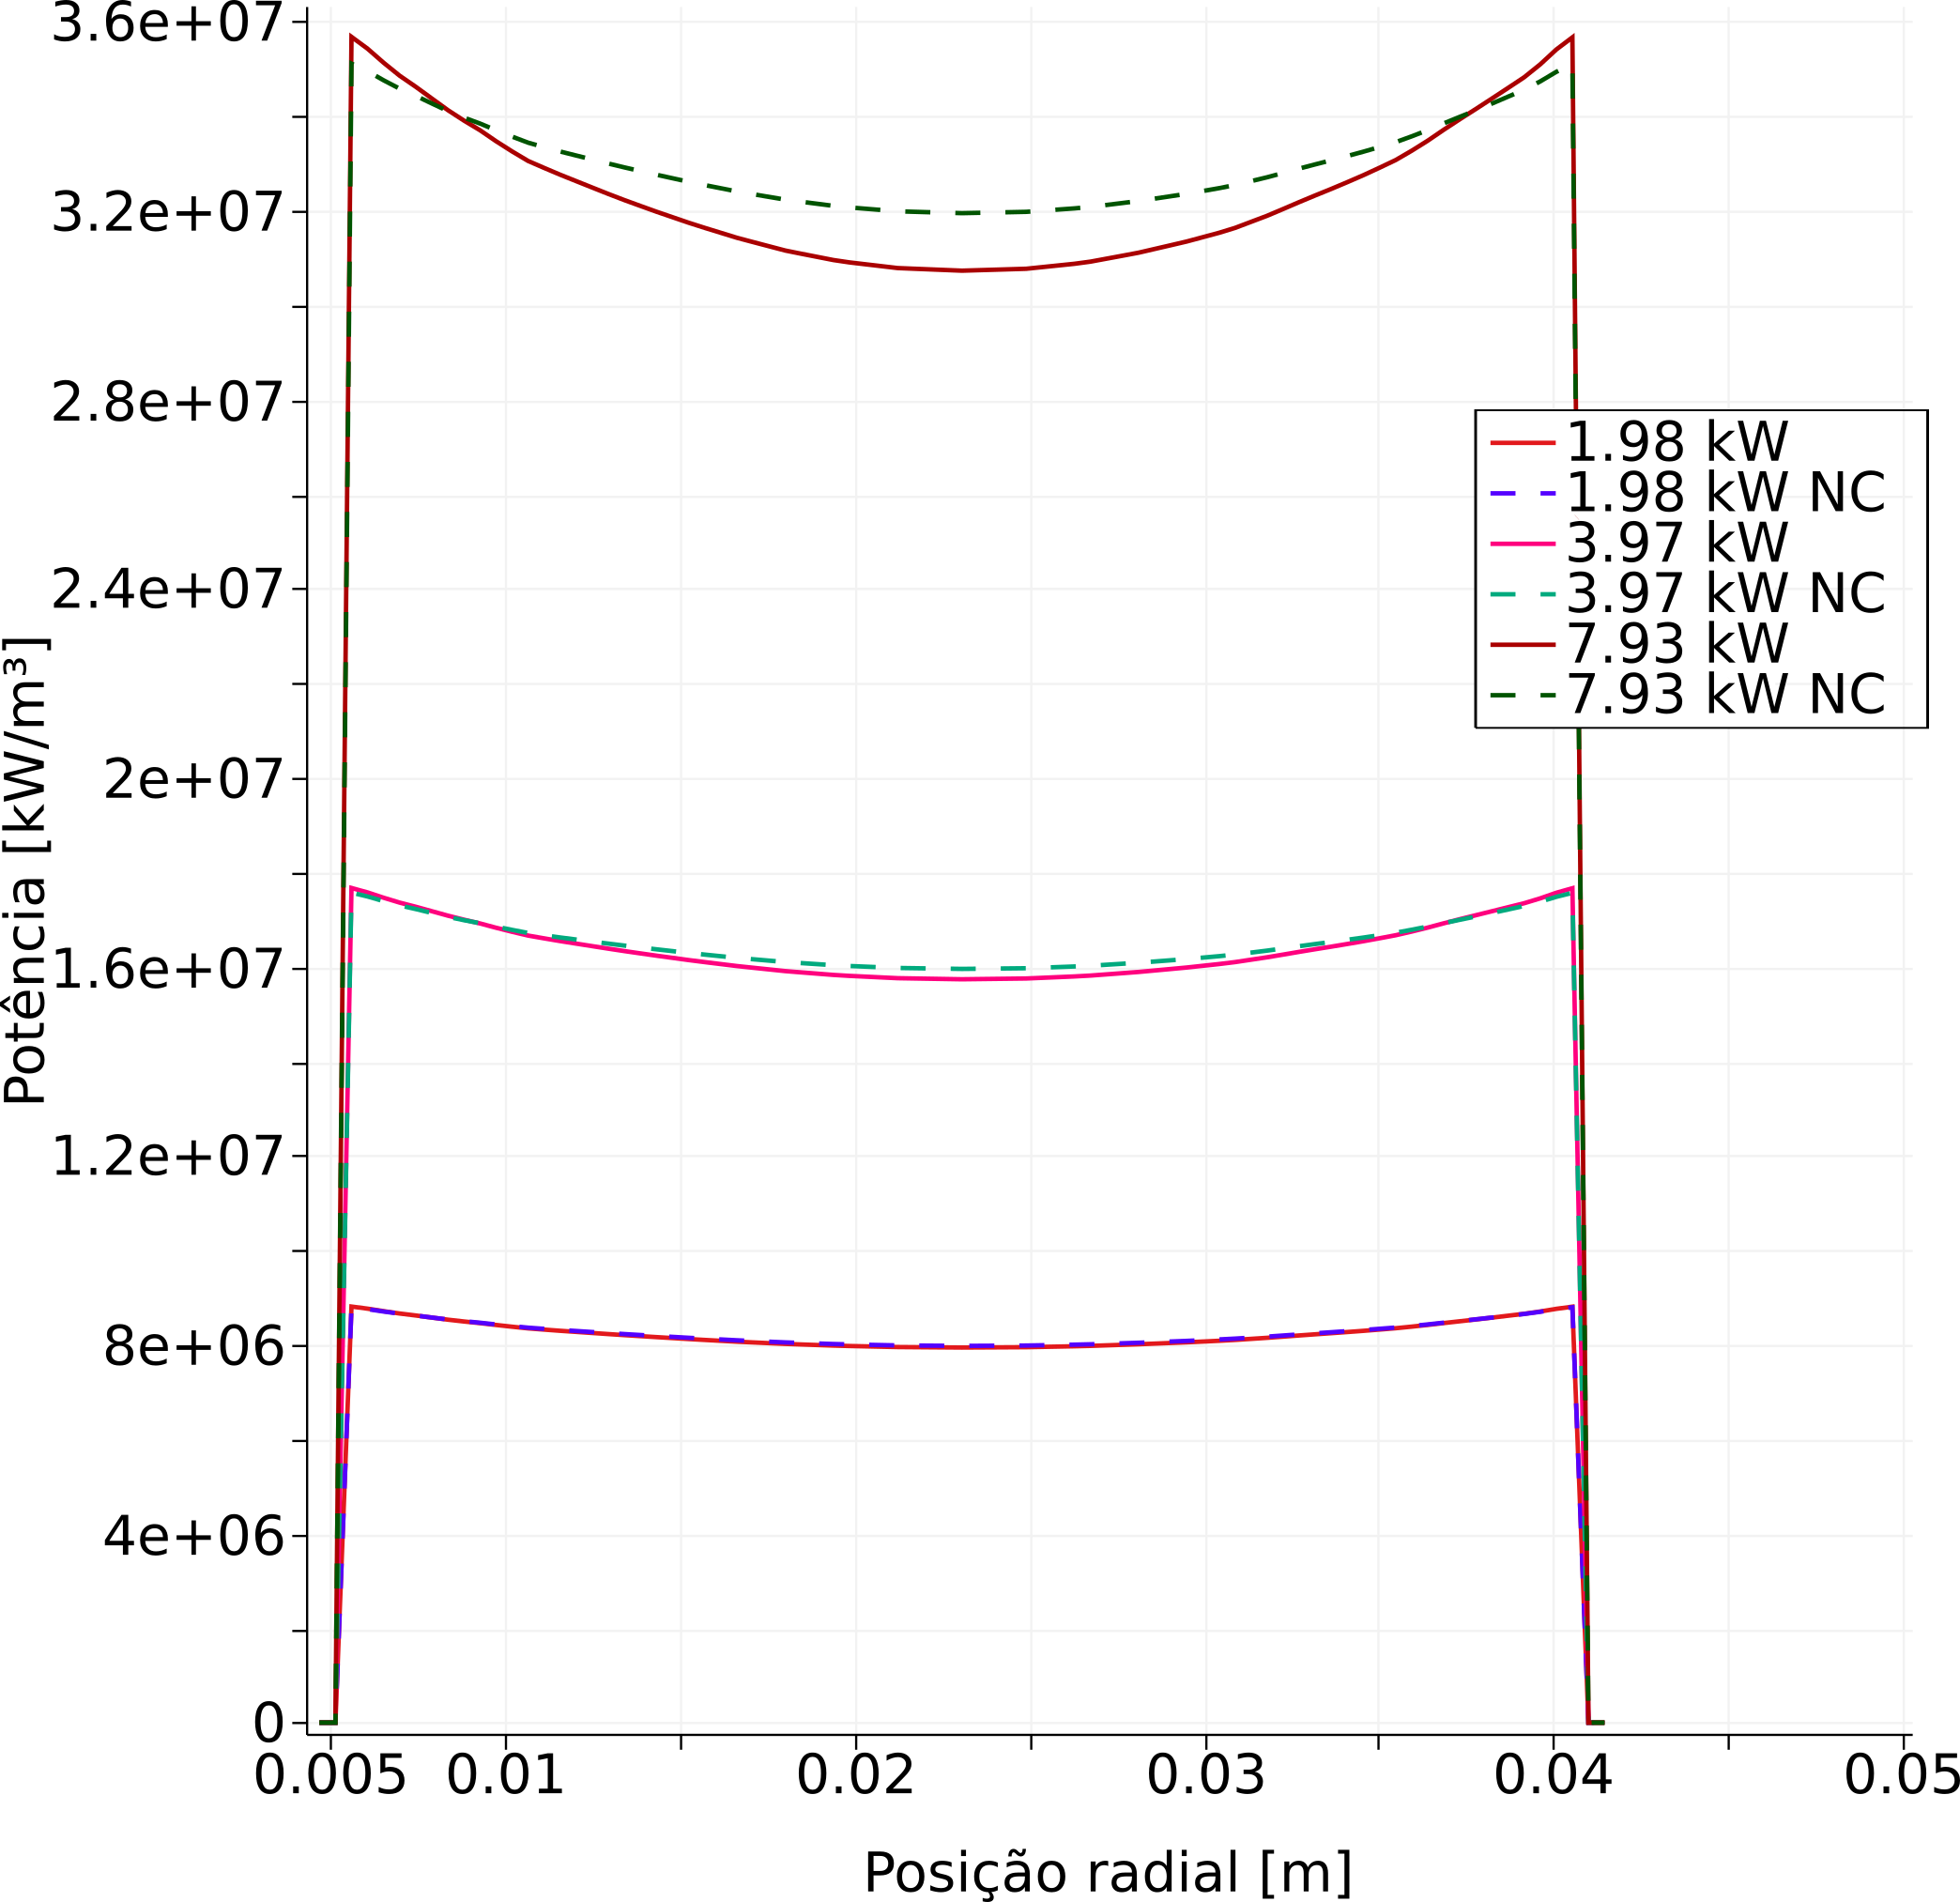
\includegraphics[width=\textwidth, height=7.0cm]{../figuras/Q_all_x_square_port.png}
  \label{fig:keff50}
\end{frame}

%-------------------------------------------------
\subsection{Gráficos}
\begin{frame}
  \frametitle{Resultados}
  \framesubtitle{Temperatura: distribuição axial}
%  Distribuição de temperaturas [$K$].
  \centering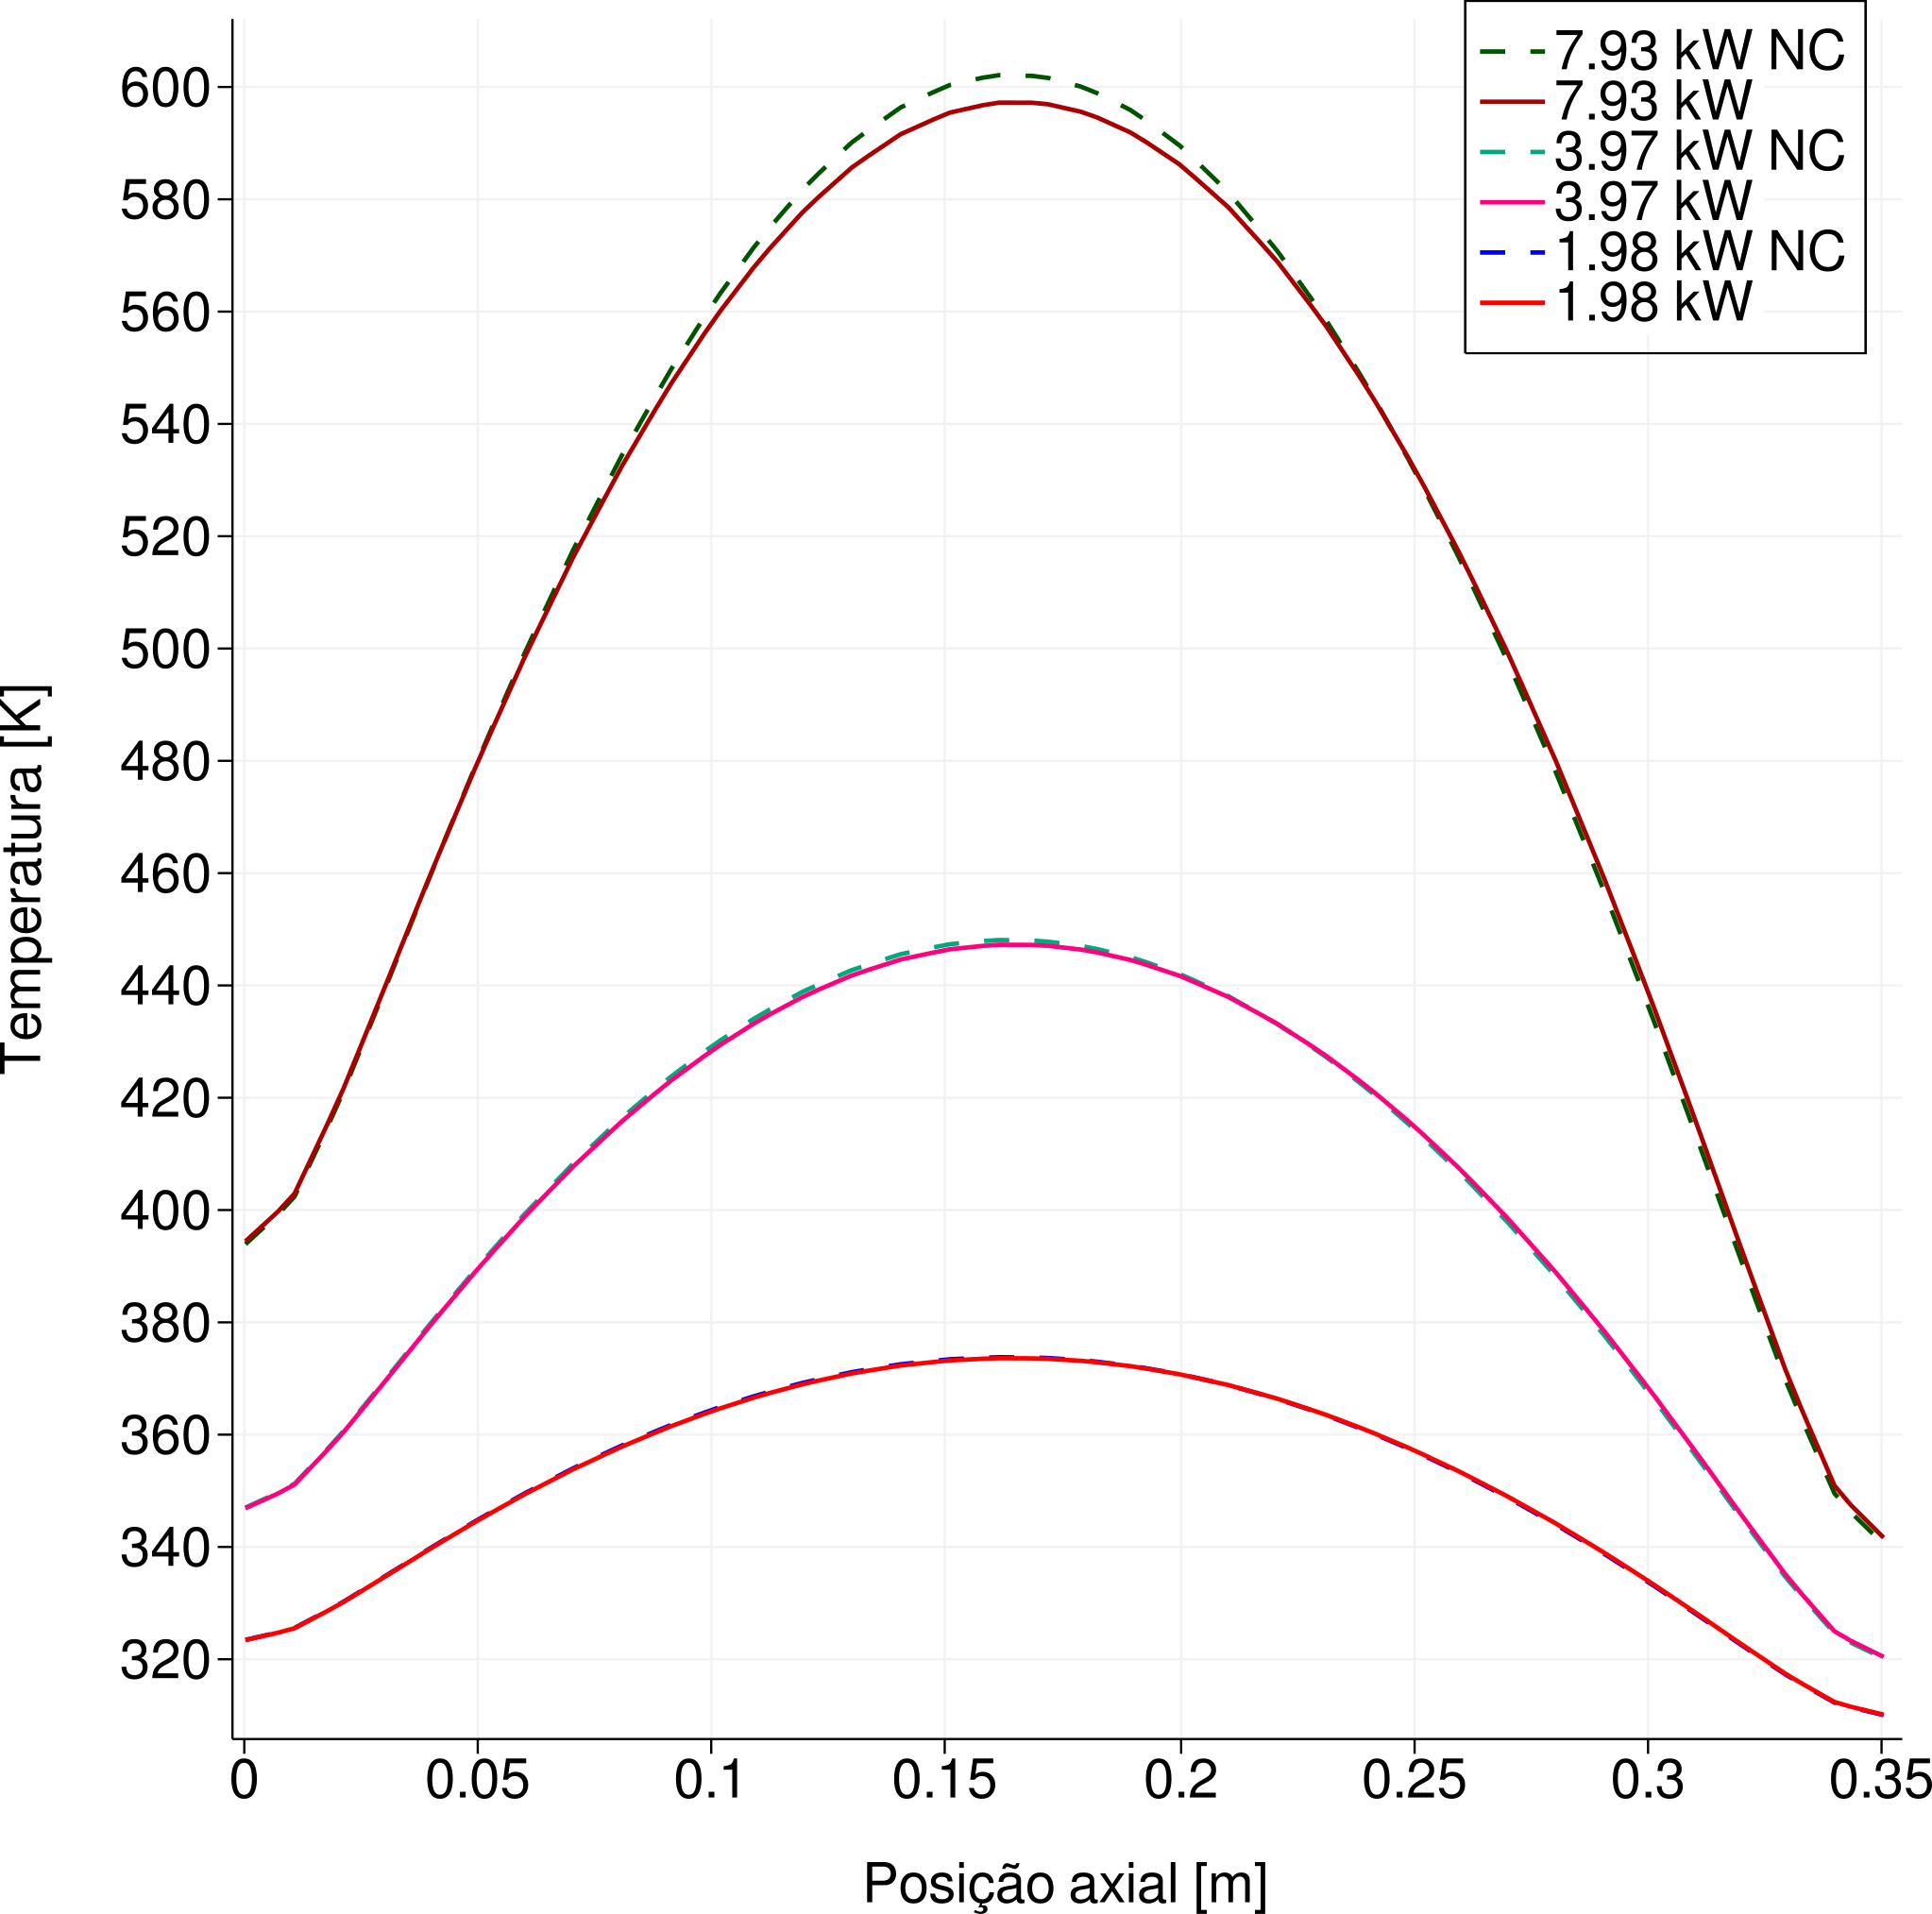
\includegraphics[width=\textwidth, height=7.0cm]{../figuras/T_z_all_square_port.png}
  \label{fig:keff50}
\end{frame}

%-------------------------------------------------
\subsection{Gráficos}
\begin{frame}
  \frametitle{Resultados}
  \framesubtitle{Temperatura: distribuição radial}
%  Distribuição de temperaturas [$K$].
  \centering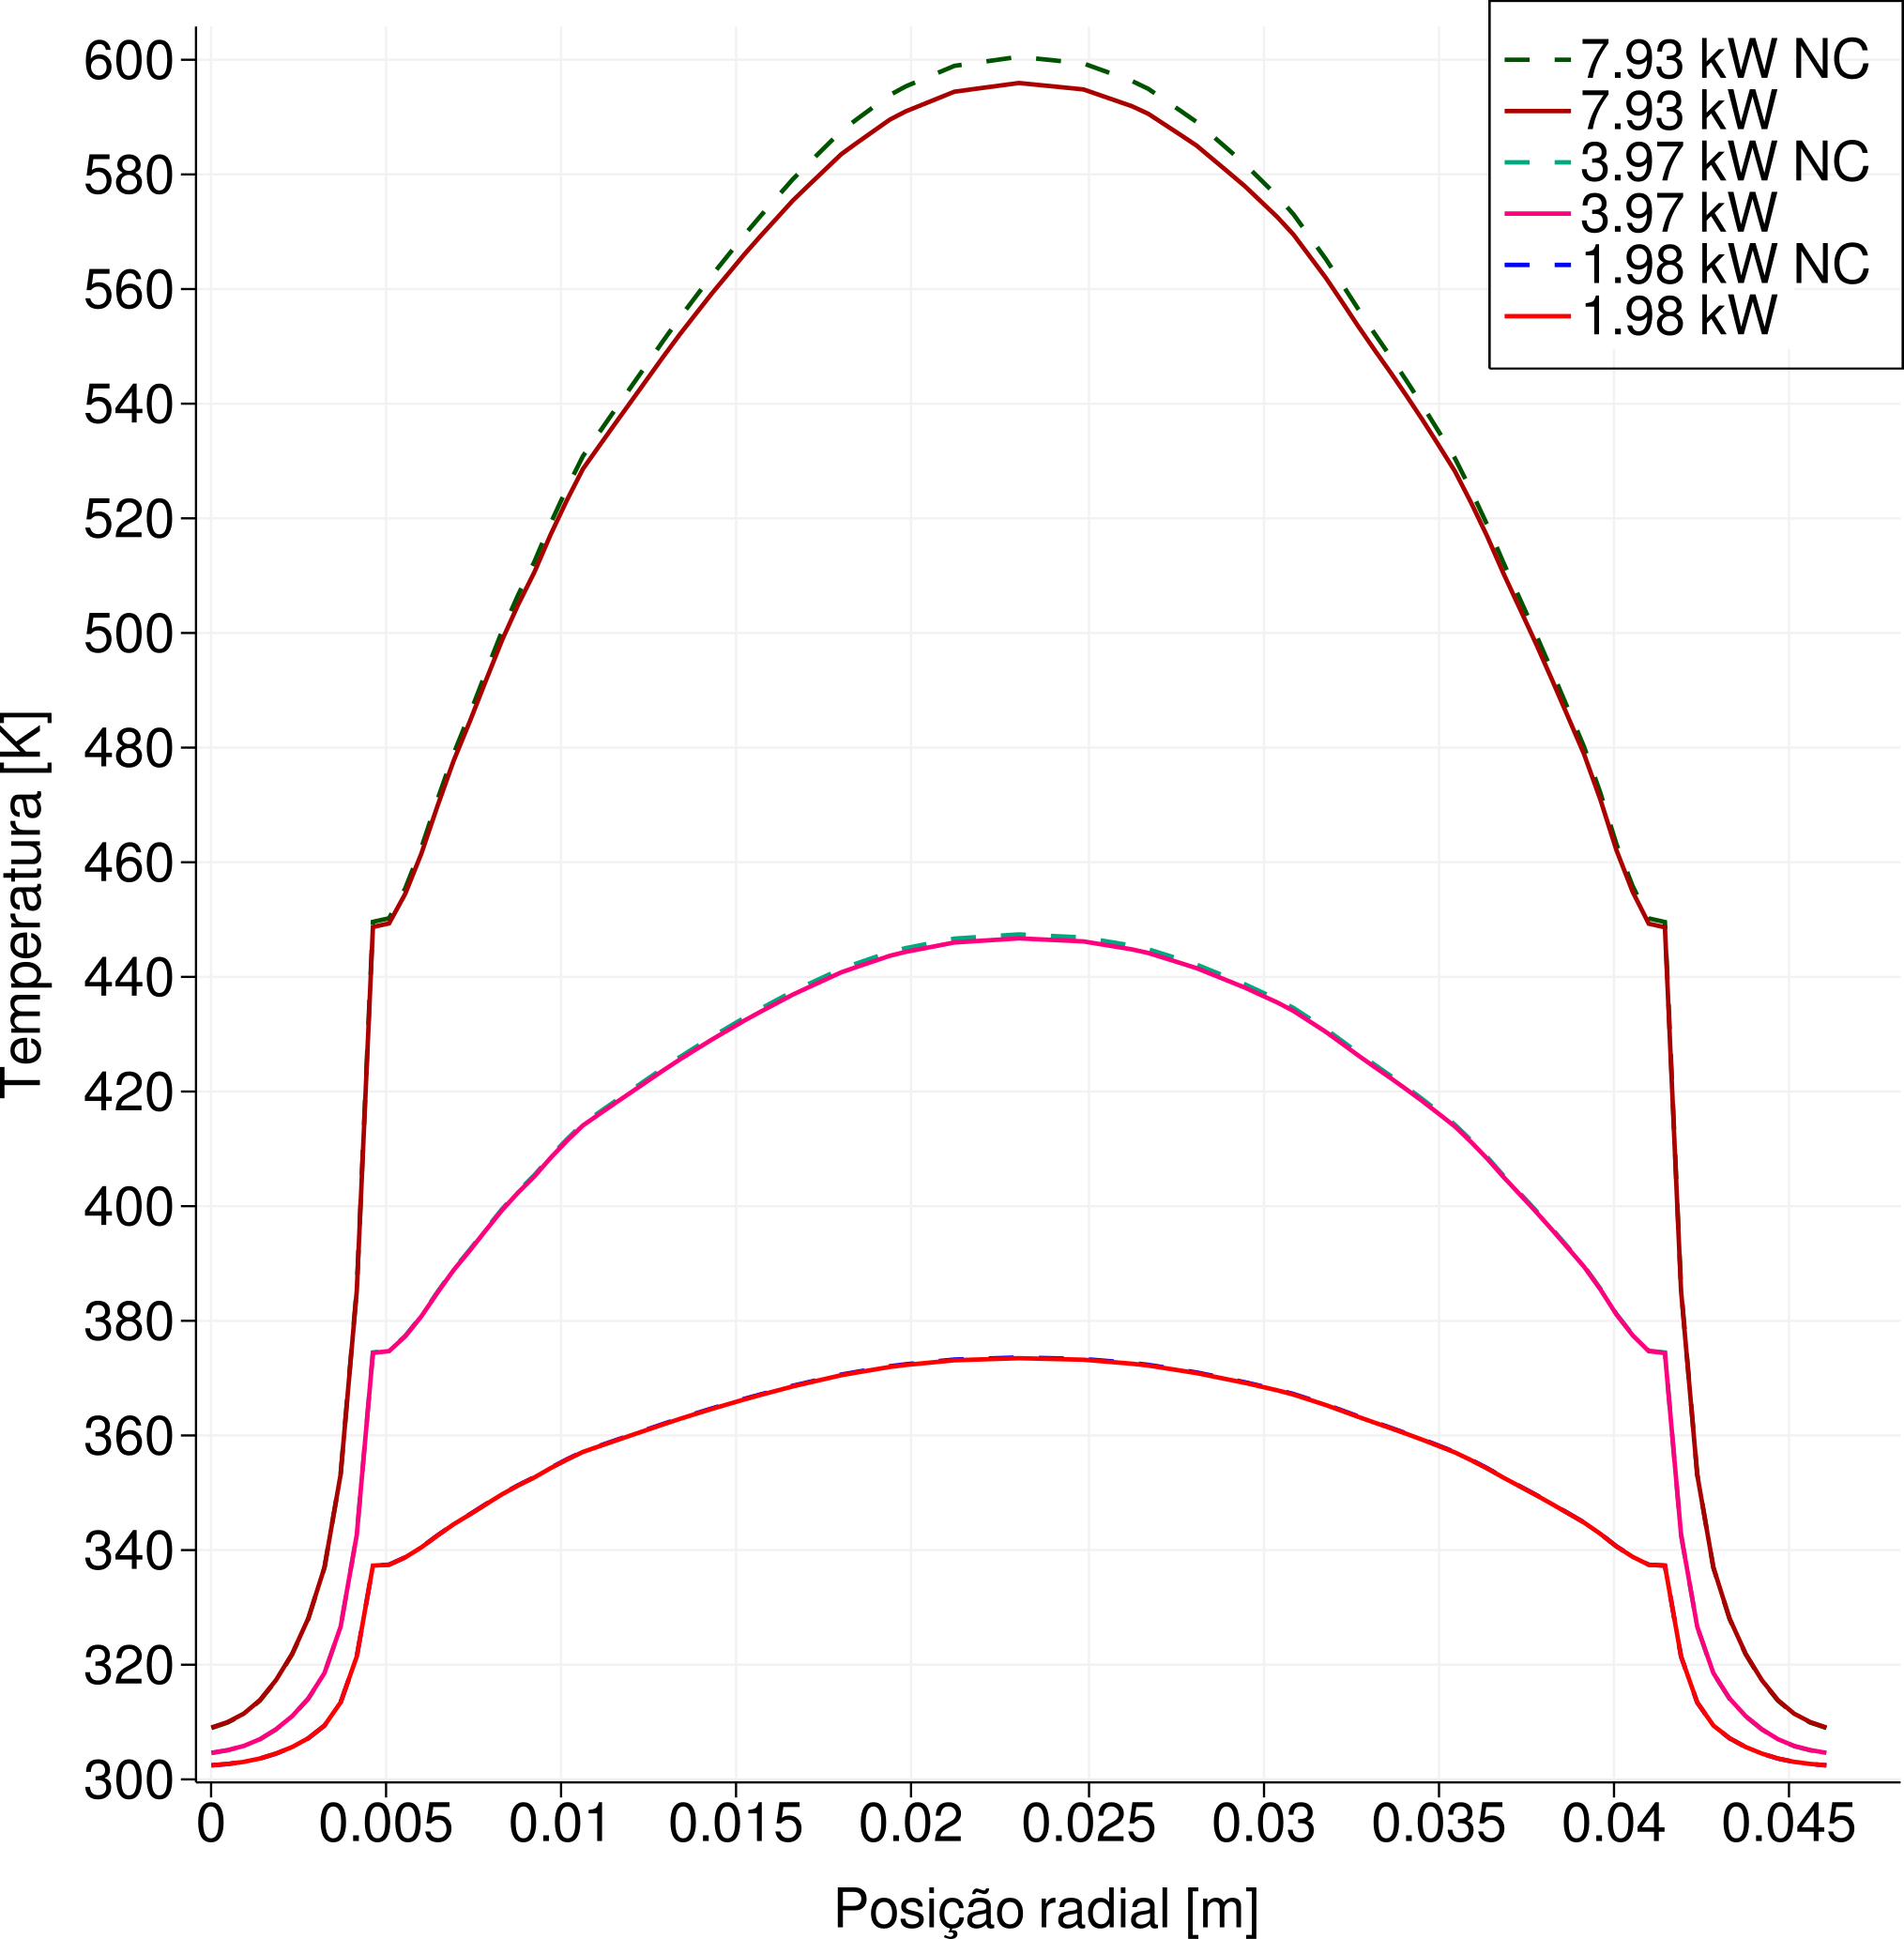
\includegraphics[width=\textwidth, height=7.0cm]{../figuras/T_x_all_square_port.png}
  \label{fig:keff50}
\end{frame}

%-------------------------------------------------
\subsection{Gráficos}
\begin{frame}
  \frametitle{Resultados}
  \framesubtitle{Convergência}
  Variação dos fatores de multiplicação efetivo ($k_{eff}$).
  \centering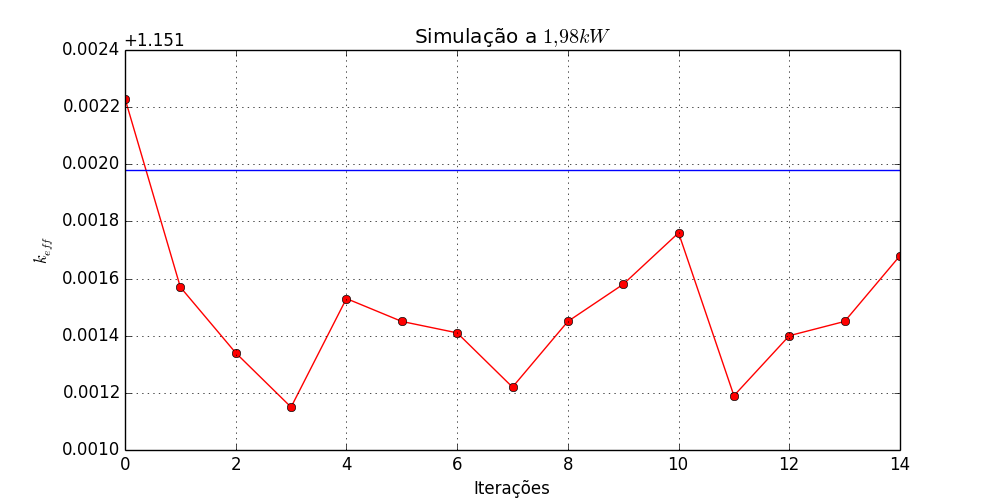
\includegraphics[scale=0.45]{../figuras/plot50.png}
  \label{fig:keff50}
\end{frame}

%-------------------------------------------------
\begin{frame}
  \frametitle{Resultados}
  \framesubtitle{Convergência}
  Variação dos fatores de multiplicação efetivo ($k_{eff}$).
  \centering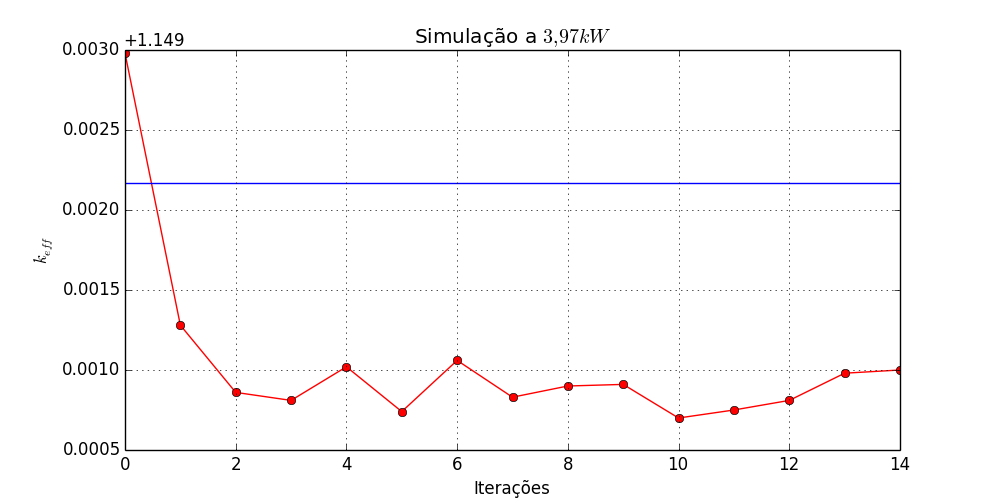
\includegraphics[scale=0.45]{../figuras/plot100.png}
  \label{fig:keff100}
\end{frame}

%-------------------------------------------------
\begin{frame}
  \frametitle{Resultados}
  \framesubtitle{Convergência}
  Variação dos fatores de multiplicação efetivo ($k_{eff}$).
  \centering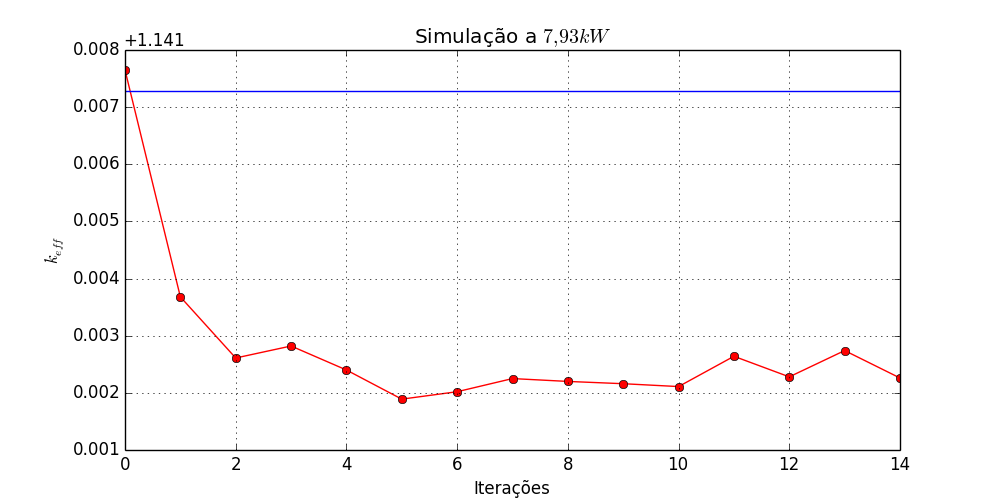
\includegraphics[scale=0.45]{../figuras/plot200.png}
  \label{fig:keff200}
\end{frame}




%-------------------------------------------------
\subsection{Fator de multiplicação}
\begin{frame}
  \frametitle{Resultados}
  \framesubtitle{Fator de multiplicação}
\begin{table}[]
\centering
%\caption{My caption}
\begin{tabular}{l|r|r|r|}
\cline{2-4}
\multicolumn{1}{c|}{}          & \multicolumn{3}{c|}{$k_{eff}$}                                                                                                                                              \\ \hline
\multicolumn{1}{|c|}{Potência} & \multicolumn{1}{c|}{Não acoplado} & \multicolumn{1}{c|}{\begin{tabular}[c]{@{}c@{}}Acoplado\\ (média durante \\os cálculos)\end{tabular}} & \multicolumn{1}{c|}{Desvio padrão} \\ \hline
\multicolumn{1}{|l|}{1,98 kW}  & 1,15298                           & 1,15249                                                                                             & 0,000257                           \\ \hline
\multicolumn{1}{|l|}{3,97 kW}  & 1,15117                           & 1,15004                                                                                             & 0,000538                           \\ \hline
\multicolumn{1}{|l|}{7,93 kW}  & 1,14829                           & 1,14378                                                                                             & 0,001367                           \\ \hline
\end{tabular}
\end{table}
\end{frame}

%-------------------------------------------------
\begin{frame}
  \frametitle{Resultados}
  \framesubtitle{Robustez(?)}
  Variação do fator de multiplicação efetivo ($k_{eff}$) com mudanças em parâmetros de convergência.
  \centering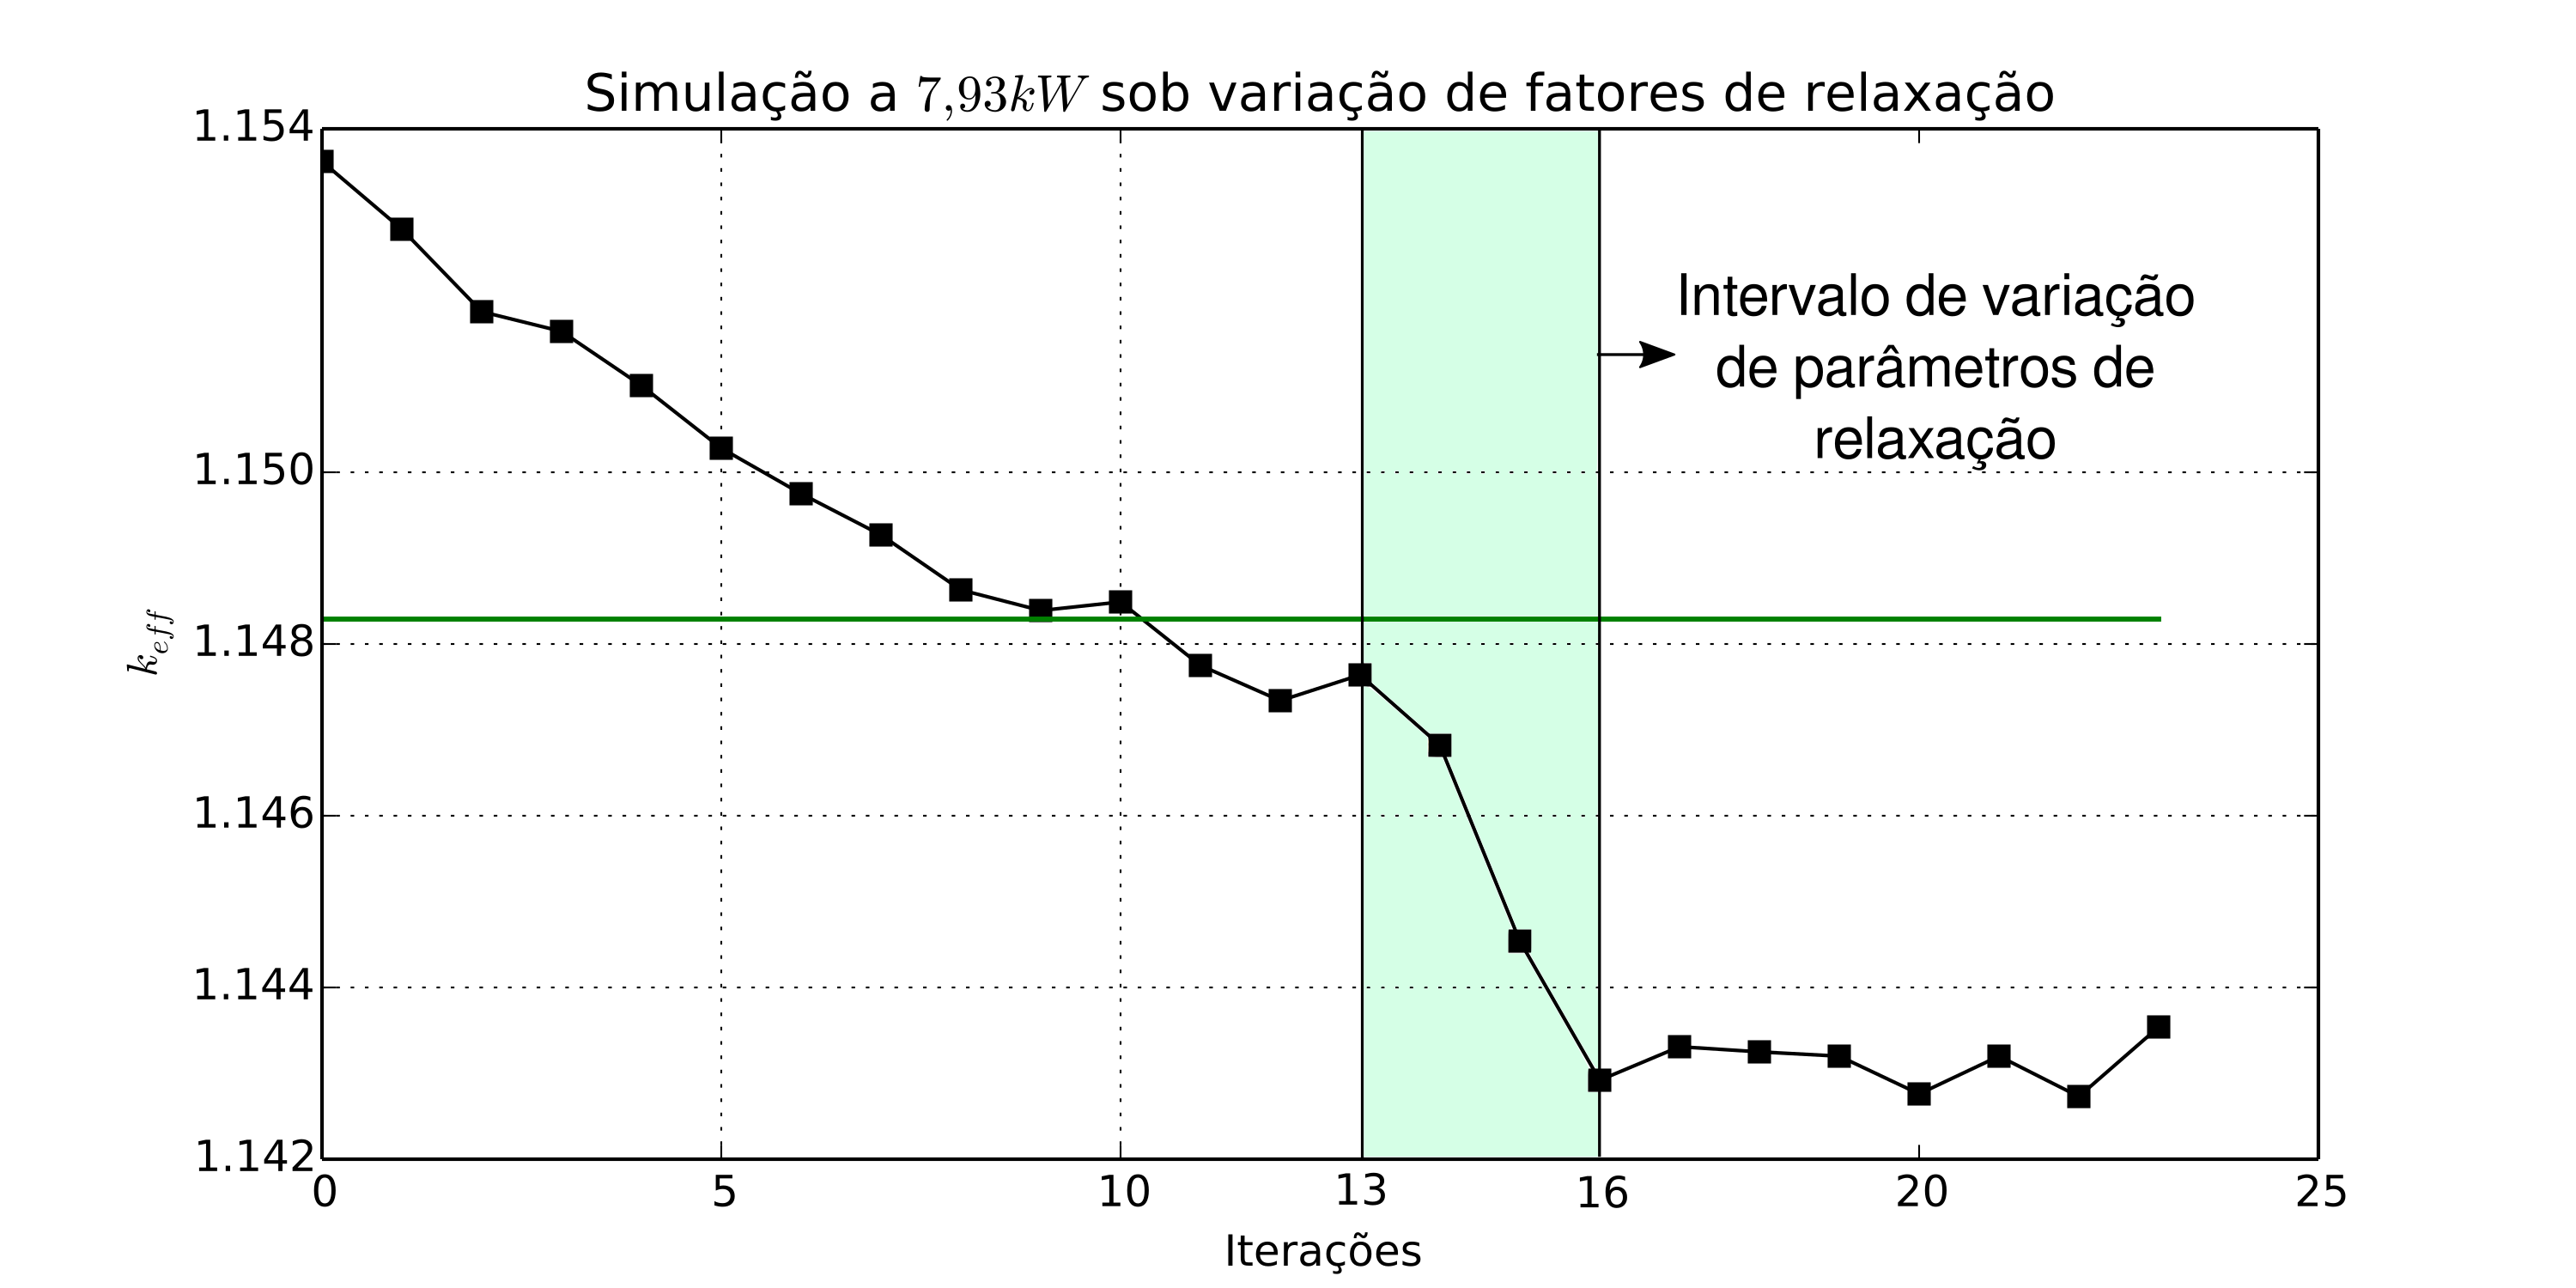
\includegraphics[scale=0.45]{../figuras/plot200-disturb-port.png}
  \label{fig:keff_dist}
%  \legend{Fonte: autor}
\end{frame}

\section{Conclusões}
%-------------------------------------------------
\begin{frame}
  \frametitle{Conclusões}
  \framesubtitle{}
\end{frame}

%-------------------------------------------------
% Frame escondido
\begin{frame}[noframenumbering]
  \frametitle{Respostas}
  \framesubtitle{Seções de choque}
  Teste
\end{frame}



\end{document}
